%%%%%%%%%%%%%%%%%%%%%%%%%%%%%%%%%%%%%%%%%%%%%%%
\chapter{Combinatorial Results} \label{chap:comb_res}
%%%%%%%%%%%%%%%%%%%%%%%%%%%%%%%%%%%%%%%%%%%%%%%

This section contains new results on gaps of 3 different instances
of the GCN. In previous studies \cite{Wachter-Zeh:2018}, no general
vector solution outperforming scalar network coding was found for
multicast networks with $h=3$ messages. Hence, we start with a probabilistic
argument to prove that there exists a vector solution outperforming
the optimal linear solution for the $\left(\epsilon=1,\ell=1\right)-\mathcal{N}_{h=3,r,s=4}$
network. Our approach is to study the network as an matrix channel
introduced in Section \ref{subsec:Matrix-channel} and apply the Symmetric
Lov\'asz local lemma (LLL) for the proof. The idea of this approach
for the vector network coding was proposed by Mosche Schwarz \cite{MosheSchwartz:2018}.
The optimal scalar linear solution was studied in \cite{Wachter-Zeh:2018}.
We therefore can compute a gap in alphabet sizes for our vector solutions
and the optimal scalar linear solution in Section \ref{sec:Network_e1l1h3rs4}. 

Then, we generalize the proof to the $\left(\epsilon=1,\ell=1\right)-\mathcal{N}_{h,r,s}$
network, the $\left(\epsilon>1,\ell=1\right)-\mathcal{N}_{h,r,s}$
network and the $\left(\epsilon=1,\ell>1\right)-\mathcal{N}_{h=2\ell,r,s=2\ell+1}$
network. As explained in Section \ref{sec:What-is-NC}, multiple parallel
links $\ell$ of a data unit help us to show networks with large-capacity
transmission between source and receivers. The direct links among
them are not really usual in reality, i.e. a server and a client often
has long-distance connection through multiple intermediate nodes,
it is thus interesting to study networks with $\epsilon=1$ and $l>1$.
By applying rank requirements for each receiver to be able to solve
linear systems in (\ref{eq:linear_system}), we prove that there exists
scalar and vector solutions for such networks if the number $r$ of
intermediate nodes is bounded by a certain number. Then, we can show
gaps of the networks based network parameters $q,t,\alpha,h$. In
this study, we derive lower bounds on such gaps following to Sectioin
\ref{subsec:Comparison-between-scalar-and-vector-sol}, our gap for
the $\left(\epsilon=1,\ell>1\right)-\mathcal{N}_{h=2\ell,r,s=2\ell+1}$
network is thus less than the one found in \cite{Wachter-Zeh:2018}.
However, gaps for the $\left(\epsilon=1,\ell=1\right)-\mathcal{N}_{h,r,s}$
network and the $\left(\epsilon>1,\ell=1\right)-\mathcal{N}_{h,r,s}$
network are not known in any other studies.

We formally use $r_{\mathrm{scalar}}$ and $r_{\mathrm{vector}}$
in Table \ref{tab:Parameters-of-network} to distinguish the $r$
parameter of GCN for scalar solutions and vector solutions to compare
a gap derived from such solutions. Because they both have the same
meaning as a number of intermediate nodes in a network, we use $r$
when we need to state a vector solution or a scalar solution exists
under some conditions of $r$.

\section{$\left(\epsilon=1,\ell=1\right)-\mathcal{N}_{h=3,r,s=4}$ Network
\label{sec:Network_e1l1h3rs4}}

\begin{figure}[H]
\caption{The $(\epsilon=1,\ell=1)-\mathcal{N}_{h=3,r,s=4}$ network\label{fig:nw_e1_l1_h3_r_s4}}

\centering{}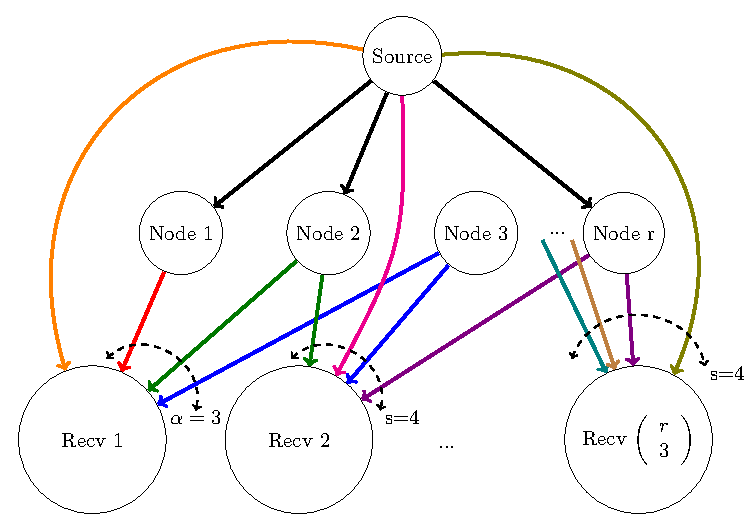
\includegraphics[width=0.5\paperwidth]{./figures/nw_e1_l1_h3_r_s4}
\end{figure}

In this subsection, we derive a lower bound on the maximum number
of receivers for the $\left(\epsilon=1,\ell=1\right)-\mathcal{N}_{h=3,r,s=4}$
network such that a vector solution for the network exists. Due to
$\alpha=3$, the number of receivers is $N=\left(\begin{array}{c}
r\\
3
\end{array}\right)$ by definition in Section \ref{sec:Description_GCN}. A problem of
finding the maximum $N$ is thus equivalent to find a maximum number
of intermediate nodes $r$. We denote the maximum number of such nodes
for a vector solution by $r_{\mathrm{max,vector}}$. Our goal is therefore
to derive $r_{\mathrm{max,vector}}$ such that there exists a vector
solution for the $\left(1,1\right)-\mathcal{N}_{3,r,4}$ network for
any $r\leq r_{\mathrm{max,vector}}$. In \cite[Section VIII.C]{Wachter-Zeh:2018},
Etzion and Wachter-Zeh stated that there exists a scalar solution
for the network for any $r\leq r_{\mathrm{max,scalar}}$ with $r_{\mathrm{max,scalar}}=2\left(q_{s}^{2}+q_{s}+1\right)$.
Based on $r_{\mathrm{max,scalar}}$ and $r_{\mathrm{max,vector}}$,
we then calculate the gap in alphabet sizes for such scalar and vector
solutions of the $\left(1,1\right)-\mathcal{N}_{3,r,4}$ network following
to Section \ref{subsec:Comparison-between-scalar-and-vector-sol}.
To discuss the vector solvability of the network, we introduce a rank
requirement on the transfer matrix $\boldsymbol{A}_{j}$ corresponding
to each receiver $R_{j}$. In Figure \ref{fig:nw_e1_l1_h3_r_s4},
each receiver $R_{j}$ obtains 4 linear combinations of the 3 source
messages. In other words, the transfer matrix $\boldsymbol{A}_{j}$
maps the messages $x_{1},x_{2},x_{3}$ to $y_{j}^{\left(1\right)},y_{j}^{\left(2\right)},y_{j}^{\left(3\right)},y_{j}^{\left(4\right)}$
or $\boldsymbol{x}_{1},\boldsymbol{x}_{2},\boldsymbol{x}_{3}$ to
$\boldsymbol{y}_{j}^{\left(1\right)},\boldsymbol{y}_{j}^{\left(2\right)},\boldsymbol{y}_{j}^{\left(3\right)},\boldsymbol{y}_{j}^{\left(4\right)}$
respectively regarding to scalar or vector network coding, which are
illustrated as linear systems of equations for $R_{1}$ in Figure
\ref{fig:rk_h3}. Both $r_{\mathrm{scalar}}$ and $r_{\mathrm{vector}}$
indicate the number of nodes $r$ and we mostly use $r$ in this subsection
for ease of notation.

\begin{figure}[H]
\caption{The vector network coding of $(\epsilon=1,l=1)-\mathcal{N}_{h=3,r,s=4}$
represents as a matrix problem \label{fig:rk_h3}}

\centering{}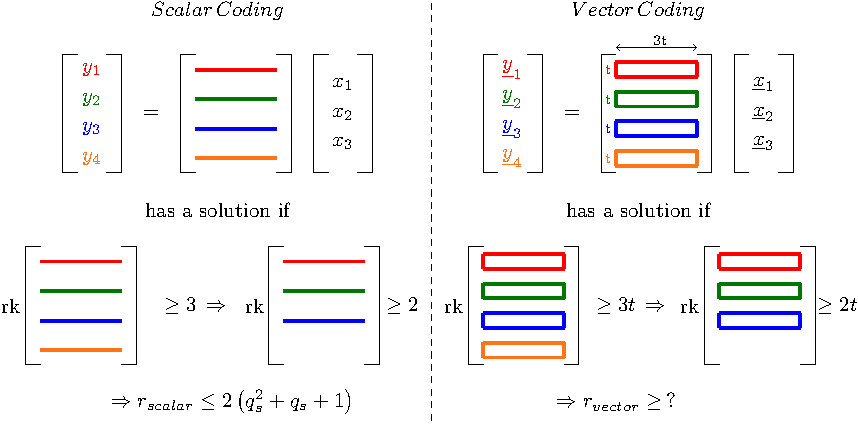
\includegraphics[width=0.6\paperwidth]{./figures/rk_h3}
\end{figure}

Following to (\ref{eq:linear_system}), each receiver $R_{j}$ has
to solve a linear equation system of $3t$ variables with $4t$ equations
to recover $h=3$ messages as below:
\begin{equation}
\left[\begin{array}{c}
\boldsymbol{y}_{j}^{\left(1\right)}\\
\boldsymbol{y}_{j}^{\left(2\right)}\\
\boldsymbol{y}_{j}^{\left(3\right)}\\
\boldsymbol{y}_{j}^{\left(4\right)}
\end{array}\right]=\boldsymbol{A}_{j}\cdot\underline{x}=\left[\begin{array}{c}
\boldsymbol{A}^{\left(r_{1}\right)}\\
\boldsymbol{A}^{\left(r_{2}\right)}\\
\boldsymbol{A}^{\left(r_{3}\right)}\\
\boldsymbol{B}^{\left(\epsilon\left(j-1\right)+1\right)}
\end{array}\right]\cdot\left[\begin{array}{c}
\boldsymbol{x}_{1}\\
\boldsymbol{x}_{2}\\
\boldsymbol{x}_{3}
\end{array}\right],\label{eq:linear_system_h3rs4}
\end{equation}
with $\boldsymbol{x}_{1},\ldots,\boldsymbol{x}_{3}\in\ensuremath{\mathbb{F}}_{q}^{t},\boldsymbol{y}_{j}^{\left(1\right)},\ldots,\boldsymbol{y}_{j}^{\left(4\right)}\in\ensuremath{\mathbb{F}}_{q}^{t},\boldsymbol{A}^{\left(r_{v}\right)},\in\ensuremath{\mathbb{F}}_{q}^{t\times3t}$
for $v=1,\ldots,3$ and $1\leq r_{1}<r_{2}<r_{3}\leq r$, and $\boldsymbol{B}^{\left(\epsilon\left(j-1\right)+1\right)}\in\ensuremath{\mathbb{F}}_{q}^{t\times3t}$
for $j\in\left\{ 1,\ldots,\left(\begin{array}{c}
r\\
3
\end{array}\right)\right\} $.

The network is solvable, if $\boldsymbol{A}_{j}$ has full-rank:
\[
\mathrm{rk}\left[\begin{array}{c}
\boldsymbol{A}_{j}^{\left(r_{1}\right)}\\
\boldsymbol{A}_{j}^{\left(r_{2}\right)}\\
\boldsymbol{A}_{j}^{\left(r_{3}\right)}\\
\boldsymbol{B}^{\left(\epsilon\left(j-1\right)+1\right)}
\end{array}\right]\geq3t.
\]

Since coding coefficients for $\boldsymbol{B}^{\left(\epsilon\left(j-1\right)+1\right)}$
can be independently chosen for any receiver $R_{j}$, there always
exists $\boldsymbol{B}^{\left(\epsilon\left(j-1\right)+1\right)}$
such that,
\begin{equation}
\mathrm{rk}\left[\begin{array}{c}
\boldsymbol{A}^{\left(r_{1}\right)}\\
\boldsymbol{A}^{\left(r_{2}\right)}\\
\boldsymbol{A}^{\left(r_{3}\right)}
\end{array}\right]\geq2t,\label{eq:rk_rqm_e1l1h3s4}
\end{equation}
if and only if $\mathrm{rk}\left[\boldsymbol{A}_{j}\right]\geq3t$.

We formalize the problem by an approach with Lov\'asz local lemma,
which was initially proposed by Schwartz in \cite{MosheSchwartz:2018}.

Let $\mathcal{E}_{r_{1},r_{2},r_{3}}$ be an event that a receiver
$R_{j}$ is assigned a transfer matrix $\boldsymbol{A}_{j}$such that
$\mathrm{rk}\left[\begin{array}{c}
\boldsymbol{A}^{\left(r_{1}\right)}\\
\boldsymbol{A}^{\left(r_{2}\right)}\\
\boldsymbol{A}^{\left(r_{3}\right)}
\end{array}\right]<2t$, i.e.,

\[
\mathcal{E}_{r_{1},r_{2},r_{3}}=\left\{ \mathrm{rk}\left[\begin{array}{c}
\boldsymbol{A}^{\left(r_{1}\right)}\\
\boldsymbol{A}^{\left(r_{2}\right)}\\
\boldsymbol{A}^{\left(r_{3}\right)}
\end{array}\right]<2t\right\} ,
\]

for $1\leq r_{1}<r_{2}<r_{3}\leq r$ and $\boldsymbol{A}^{\left(r_{1}\right)},\ldots,\boldsymbol{A}^{\left(r_{3}\right)}\in\ensuremath{\mathbb{F}}_{q}^{t\times3t}$,
chosen idenpendently and uniformly random.
\begin{lem}[Symmetric Lov\'asz local lemma (LLL) \cite{Schwarz:2013}]
 A set of events $\mathcal{E}_{i}$, such that each event occurs
with probability at most $p$. If each event is independent of all
others except for at most $d$ of them and $4pd\leq1$, then: $\mathrm{Pr}\left[\stackrel[i=1]{n}{\bigcap}\overline{\mathcal{E}}_{i}\right]>0$.
\label{thm:LLL}
\end{lem}
In \cite{Overbeck:2007}, the number of $\left[n\times m\right]$
matrices of rank $i$ over $\ensuremath{\mathbb{F}}_{q}$ is given,

\begin{equation}
\mathrm{NM}_{i,n,m}=\stackrel[j=0]{i-1}{\mathop{\prod}}\frac{\left(q^{m}-q^{j}\right)\left(q^{n}-q^{j}\right)}{q^{i}-q^{j}}.\label{eq:num_of_rank_t_matrices}
\end{equation}

We therefore have $\mathrm{NM}_{i<2t,3t,3t}$ as the number of $\left[3t\times3t\right]$
matrices whose ranks are less than $2t$. Each event $\mathcal{E}_{r_{1},r_{2},r_{3}}$
has a probability calculated by dividing $\mathrm{NM}_{i<2t,3t,3t}$
by $q^{9t^{2}}$, where $q^{9t^{2}}$ is the number of all possible
$\left[3t\times3t\right]$ matrices over $\ensuremath{\mathbb{F}}_{q}$.
The probability is bounded as stated in Lemma \ref{lem:prob_p_LLL_formula}.
\begin{lem}
\label{lem:prob_p_LLL_formula} If $\mathrm{Pr}\left[\mathcal{E}_{r_{1},r_{2},r_{3}}\right]\leq p$,
then,
\[
p\in\Theta\left(q^{-t^{2}-2t-1}\right),\forall t\geq2.
\]
\end{lem}
\begin{proof}
Following to (\ref{eq:rk_rqm_e1l1h3s4}), a event $\mathcal{E}_{r_{1},r_{2},r_{3}}$
occurs when $\mathrm{rk}\left[\boldsymbol{A}_{j}\right]<3t$, and
its probability is bounded by $p$ (with $0\leq p\leq1$) as following,
\begin{eqnarray}
\mathrm{Pr}\left[\mathcal{E}_{r_{1},r_{2},r_{3}}\right]=\mathrm{Pr}\left[\mathrm{rk}\left[\begin{array}{c}
\boldsymbol{A}^{\left(r_{1}\right)}\\
\boldsymbol{A}^{\left(r_{2}\right)}\\
\boldsymbol{A}^{\left(r_{3}\right)}
\end{array}\right]<2t\right] & = & \stackrel[i=0]{2t-1}{\mathop{\sum}}\mathrm{Pr}\left[\mathrm{rk}\left[\begin{array}{c}
\boldsymbol{A}_{j}^{\left(r_{1}\right)}\\
\boldsymbol{A}_{j}^{\left(r_{2}\right)}\\
\boldsymbol{A}_{j}^{\left(r_{3}\right)}
\end{array}\right]=i\right]\label{eq:p_in_LLL}\\
 & \overset{1}{=} & \stackrel[i=0]{2t-1}{\mathop{\sum}}\frac{\mathrm{NM}_{i,3t,3t}}{q^{\left(3t\right)\cdot\left(3t\right)}}\nonumber \\
 & = & \stackrel[i=0]{2t-1}{\mathop{\sum}}\frac{\stackrel[j=0]{i-1}{\mathop{\prod}}\frac{\left(q^{3t}-q^{j}\right)^{2}}{q^{i}-q^{j}}}{q^{9t^{2}}}.\label{eq:p_eq_h3}
\end{eqnarray}

(1): Applying \ref{eq:num_of_rank_t_matrices} for $\left[3t\times3t\right]$
matrices over $\ensuremath{\mathbb{F}}_{q}$ of rank $i=0,\ldots,2t-1$.

In the following, we view $\stackrel[j=0]{i-1}{\mathop{\prod}}\frac{\left(q^{3t}-q^{j}\right)^{2}}{q^{i}-q^{j}}$
as a polynomial in $q$.

We consider the numerator of (\ref{eq:p_eq_h3}): $\stackrel[j=0]{i-1}{\mathop{\prod}}\frac{\left(q^{3t}-q^{j}\right)^{2}}{q^{i}-q^{j}}=\frac{p_{N}^{(i)}(q)}{p_{D}^{(i)}(q)}=p^{(i)}(q)$.

Due to $i$-times product and large $t$: $\left.\begin{array}{c}
\mathrm{deg}\left(p_{N}^{(i)}(q)\right)=q^{i6t}\\
\mathrm{deg}\left(p_{D}^{(i)}(q)\right)=q^{i^{2}}
\end{array}\right\} \Rightarrow p^{(i)}(q)\approx q^{i6t-i^{2}}$.

Therefore, we have: $\stackrel[i=0]{2t-1}{\mathop{\sum}}\stackrel[j=0]{i-1}{\mathop{\prod}}\frac{\left(q^{3t}-q^{j}\right)^{2}}{q^{i}-q^{j}}=\stackrel[i=0]{2t-1}{\mathop{\sum}}p^{(i)}(q)\approx\stackrel[i=0]{2t-1}{\mathop{\sum}}q^{i6t-i^{2}}$.

To maximize the sum, we set derivation of it to 0 and find the corresponding
root: 
\begin{eqnarray*}
 & \left(i6t-i^{2}\right)^{'} & =0\\
\Leftrightarrow & 6t-2i & =0\\
\Leftrightarrow & i & =3t.
\end{eqnarray*}

However, the upper limit of the sum is $\left(2t-1\right)$, which
is less than $3t$ for all $t\geq2$.
\[
\Rightarrow\mathrm{max}\left\{ q^{i6t-i^{2}}:i=0,2\ldots,2t-1\right\} =\left.q^{i6t-i^{2}}\right|_{i=2t-1}=q^{8t^{2}-2t-1}.
\]

Hence,
\[
\underset{i}{\mathrm{max}}\left\{ \stackrel[i=0]{2t-1}{\mathop{\sum}}p^{(i)}(q)\right\} \in\Theta\left(\mathrm{max}\left\{ q^{i6t-i^{2}}:i=1,2\ldots,2t-1\right\} \right)=\Theta\left(q^{8t^{2}-2t-1}\right)
\]
\[
\Rightarrow\underset{i}{\mathrm{max}}\left\{ \frac{\stackrel[i=0]{2t-1}{\mathop{\sum}}p^{(i)}(q)}{q^{9t^{2}}}\right\} \in\Theta\left(q^{-t^{2}-2t-1}\right)
\]
\[
\Rightarrow p\in\Theta\left(q^{-t^{2}-2t-1}\right)
\]
\end{proof}
Each event considered under the Local lemma \ref{thm:LLL} is not
required to be independent to all other events, and it allows some
dependence among events stated in Lemma \ref{lem:dependecy_d_LLL}.
\begin{lem}
Each event $\mathcal{E}_{r_{1},r_{2},r_{3}}$ is dependent on at most
$d\left(r\right)\leq\frac{3}{2}r^{2}$ other events. \label{lem:dependecy_d_LLL}
\end{lem}
\begin{proof}
It is clear that $\mathcal{E}_{r_{1},r_{2},r_{3}}$ is dependent on
$\mathcal{E}_{r_{1}^{'},r_{2}^{'},r_{3}^{'}}$ if and only if $\left\{ r_{1},r_{2},r_{3}\right\} \cap\left\{ r_{1}^{'},r_{2}^{'},r_{3}^{'}\right\} \neq\emptyset$.
Let us consider $\left\{ r_{1},r_{2},r_{3}\right\} \cap\left\{ r_{1}^{'},r_{2}^{'},r_{3}^{'}\right\} =\left\{ r_{1}\right\} =\left\{ r_{1}^{'}\right\} $,
we have maximum $\left(\begin{array}{c}
r-1\\
2
\end{array}\right)$ such $\mathcal{E}_{r_{1},r_{2},r_{3}}$ events. Similarly with $\left\{ r_{1},r_{2},r_{3}\right\} \cap\left\{ r_{1}^{'},r_{2}^{'},r_{3}^{'}\right\} =\left\{ r_{2}\right\} $
and $\left\{ r_{1},r_{2},r_{3}\right\} \cap\left\{ r_{1}^{'},r_{2}^{'},r_{3}^{'}\right\} =\left\{ r_{3}\right\} $,
we obtain
\[
d\left(r\right)\leq3\cdot\left(\begin{array}{c}
r-1\\
2
\end{array}\right)=3\cdot\frac{\left(r-1\right)\left(r-2\right)}{2}=\frac{3}{2}\left(r^{2}-3r+2\right)
\]
\[
\Rightarrow d\left(r\right)\leq\frac{3}{2}r^{2}
\]

Therefore, each event $\mathcal{E}_{r_{1},r_{2},r_{3}}$ is independent
of all other events except at most $d\leq\frac{3}{2}r^{2}$ of them.
\end{proof}
\begin{thm}
There is an $r_{\mathrm{max,vector}}\in\Omega\left(q^{t^{2}/2+\mathcal{O}\left(t\right)}\right)$
such that for any $r\leq r_{\mathrm{max,vector}}$ there exists a
vector solution for the $\left(\epsilon=1,l=1\right)-\mathcal{N}_{h=3,r,s=4}$
network . \label{theo:r_for_vector_sol_e1l1h3rs4}
\end{thm}
\begin{proof}
By the intersection rule, none of the $\mathcal{E}_{r_{1},r_{2},r_{3}}$
events occuring is equivalent to an event $T$ whose set of outcomes
satisfy (\ref{eq:rk_rqm_e1l1h3s4}) as following,
\[
T=\stackrel[i=1]{n}{\bigcap}\overline{\mathcal{E}}_{i}=\left\{ \mathrm{rk}\left[\begin{array}{c}
\boldsymbol{A}^{\left(r_{1}\right)}\\
\boldsymbol{A}^{\left(r_{2}\right)}\\
\boldsymbol{A}^{\left(r_{3}\right)}
\end{array}\right]\geq2t,\forall1\leq r_{1}<r_{2}<r_{3}\leq r\right\} .
\]
The Local lemma \ref{thm:LLL} shows that $\mathrm{Pr}\left[T\right]=\mathrm{Pr}\left[\stackrel[i=1]{n}{\bigcap}\overline{\mathcal{E}}_{i}\right]>0$
if $4\cdot p\cdot d(r)\leq1,\forall r\leq r_{\mathrm{max,vector}}$.
Furthermore, we have $d\leq\frac{3}{2}r^{2}$ following to Lemma \ref{lem:dependecy_d_LLL},
which gives: $4\cdot p\cdot\frac{3}{2}r^{2}\leq1\Rightarrow r\leq\sqrt{\frac{1}{6p}}=r_{\mathrm{max,vector}}$.

By Lemma \ref{lem:prob_p_LLL_formula}, we have $p\in\Theta\left(q^{-t^{2}-2t-1}\right)$,
\[
\Rightarrow r_{\mathrm{max,vector}}\in\Omega\left(\sqrt{\frac{1}{6p}}\right)=\Omega\left(\sqrt{\frac{1}{6q^{-t^{2}-2t-1}}}\right)=\Omega\left(q^{t^{2}/2+\mathcal{O}\left(t\right)}\right).
\]
The sufficient condition of Lemma \ref{thm:LLL} is satisfied for
any $r\leq r_{\mathrm{max,vector}}\in\Omega\left(q^{t^{2}/2+\mathcal{O}\left(t\right)}\right)$.
None of the $\mathcal{E}_{r_{1},r_{2},r_{3}}$ events occurs, so there
exists a vector solution for such $r$.
\end{proof}
\begin{cor}
The $\left(\epsilon=1,\ell=1\right)-\mathcal{N}_{h=3,r,s=4}$ network
has a vector solution with a gap $q^{t^{2}/4+\mathcal{O}(t)}$.
\end{cor}
\begin{proof}
In \cite[Sec. VIII-C]{Wachter-Zeh:2018}, we have that $r_{\mathrm{max,scalar}}\in\mathcal{O}\left(q_{\mathrm{s}}^{2}\right)$,
where they proved that
\begin{equation}
r_{\mathrm{scalar}}\leq2\left[\begin{array}{c}
3\\
1
\end{array}\right]_{q_{s}}=2\left(q_{s}^{2}+q_{s}+1\right).\label{eq:r_scalar_max}
\end{equation}
Following to Section \ref{subsec:Comparison-between-scalar-and-vector-sol}
and Theorem \ref{theo:r_for_vector_sol_e1l1h3rs4}, we have the gap
size 
\begin{eqnarray}
 & r_{\mathrm{max,scalar}} & =r_{\mathrm{max,vector}}\nonumber \\
\Leftrightarrow & q_{\mathrm{s,min,from\,bound}}^{2} & =q^{t^{2}/2+\mathcal{O}(t)}\nonumber \\
\Leftrightarrow & q_{\mathrm{s,min,from\,bound}} & ^{=}q^{t^{2}/4+\mathcal{O}(t)}\nonumber \\
\Rightarrow & g_{\mathrm{lower\,bound}} & =q_{\mathrm{s,min,from\,bound}}-q_{v}=q^{t^{2}/4+\mathcal{O}(t)}\label{eq:gap_e1l1h3rs4}
\end{eqnarray}

Therefore, there exists a vector solution for the network to achieve
such gap.
\end{proof}
\begin{table}[H]
\begin{centering}
\begin{tabular}{|c|c|c|}
\hline 
t & Scalar Solution & Vector Solution\tabularnewline
\hline 
\hline 
2 & $r_{\mathrm{max,scalar}}=42$ & $r_{\mathrm{max,vector}}\geq7$\tabularnewline
\hline 
3 & $r_{\mathrm{max,scalar}}=146$ & $r_{\mathrm{max,vector}}\geq62$ \tabularnewline
\hline 
4 & $r_{\mathrm{max,scalar}}=546$ & $r_{\mathrm{max,vector}}\geq1317$\tabularnewline
\hline 
5 & $r_{\mathrm{max,scalar}}=2114$ & $r_{\mathrm{max,vector}}\geq58472$\tabularnewline
\hline 
6 & $r_{\mathrm{max,scalar}}=8322$ & $r_{\mathrm{max,vector}}>10^{6}$\tabularnewline
\hline 
\end{tabular}
\par\end{centering}
\centering{}\caption{Number of intermediate nodes $r$ for the $\left(\epsilon=1,\ell=1\right)-\mathcal{N}_{h=3,r,s=4}$
network such that scalar and vector solutions exist over $t=2,\ldots,6$.
Following to (\ref{eq:r_scalar_max}), there exists a scalar solution
for the network if and only if $r\protect\leq2\left(q_{s}^{2}+q_{s}+1\right)=r_{\mathrm{max,scalar}}$.
Following to (\ref{eq:p_eq_h3}) and Lemma (\ref{lem:dependecy_d_LLL}),
we observed that vector solutions outperforming the scalar solution
when $t\protect\geq4$. \label{tab:r_over_t}}
\end{table}

By varying $t$ in (\ref{eq:p_eq_h3}), we have the Table \ref{tab:r_over_t}.
In the Table \ref{tab:r_over_t}, the vector solution outperforms
the scalar solution when $t\geq4$ for the network $\left(\epsilon=1,\ell=1\right)-\ensuremath{N}_{h=3,r,s=4}$.
In Section \ref{sec:Main-Approach} and Section \ref{sec:Alternative-Approaches}
for computational results of the network, we show vector solutions
outperforming scalar solutions in case of $t=2$ and $t=3$.


\section{$\left(\epsilon=1,\ell=1\right)-\mathcal{N}_{h,r,s}$ Network \label{sec:e1l1_nw}}

The $\left(\epsilon=1,\ell=1\right)-\mathcal{N}_{h,r,s}$ network
is a more general network compared to the $\left(\epsilon=1,\ell=1\right)-\mathcal{N}_{3,r,4}$
network studied in the previous subsection. We study a gap between
scalar and vector solutions for the $\left(1,1\right)-\mathcal{N}_{h,r,s}$
network by deriving a lower bound on the maximum number of intermediate
nodes $r$. Following to (\ref{eq:linear_system}) and an extension
of (\ref{eq:linear_system_h3rs4}), each receiver $R_{j}$ has to
solve a linear equation of $ht$ variables with $st$ equations to
recover $h$ messages as following,

\[
\left[\begin{array}{c}
\boldsymbol{y}_{j}^{\left(1\right)}\\
\vdots\\
\boldsymbol{y}_{j}^{\left(\alpha\right)}\\
\boldsymbol{y}_{j}^{\left(\alpha+1\right)}
\end{array}\right]=\boldsymbol{A}_{j}\cdot\underline{x}=\left[\begin{array}{c}
\boldsymbol{A}^{\left(r_{1}\right)}\\
\vdots\\
\boldsymbol{A}^{\left(r_{\alpha}\right)}\\
\boldsymbol{B}^{\left(j\right)}
\end{array}\right]\cdot\left[\begin{array}{c}
\boldsymbol{x}_{1}\\
\vdots\\
\boldsymbol{x}_{h}
\end{array}\right],
\]

with $\boldsymbol{x}_{1},\ldots,\boldsymbol{x}_{h}\in\ensuremath{\mathbb{F}}_{q}^{t},\boldsymbol{y}_{j}^{\left(1\right)},\ldots,\boldsymbol{y}_{j}^{\left(\alpha+1\right)}\in\ensuremath{\mathbb{F}}_{q}^{t},\boldsymbol{A}^{\left(r_{1}\right)},\ldots,\boldsymbol{A}^{\left(r_{\alpha}\right)}\in\ensuremath{\mathbb{F}}_{q}^{t\times ht}$
for $1\leq r_{1}<\ldots<r_{\alpha}\leq r$, $\boldsymbol{B}^{\left(j\right)}\in\ensuremath{\mathbb{F}}_{q}^{t\times ht}$
for $j\in\left\{ 1,\ldots,\left(\begin{array}{c}
r\\
\alpha
\end{array}\right)\right\} $.

Since coding coefficients for $\boldsymbol{B}^{\left(j\right)}$ can
be independently chosen for any receiver $R_{j}$, there always exists
$\boldsymbol{B}^{\left(j\right)}$ such that the network is solvable
with 
\[
\mathrm{rk}\left[\begin{array}{c}
\boldsymbol{A}^{\left(r_{1}\right)}\\
\vdots\\
\boldsymbol{A}^{\left(r_{\alpha}\right)}
\end{array}\right]\geq ht-t,
\]

if and only if the transfer matrix $\boldsymbol{A}_{j}$ has full
rank.

Similar to $\left(1,1\right)-\ensuremath{N}_{3,r,4}$, we apply the
Local lemma \ref{thm:LLL} for the following $\mathcal{E}_{r_{1},\ldots,r_{h-\epsilon}}$
to study the gap between scalar and vector solutions for the $\left(1,1\right)-\mathcal{N}_{h,r,s}$
network.

Let $\mathcal{E}_{r_{1},\ldots,r_{\alpha}}$ be an event that a receiver
$R_{j}$ is assigned a transfer matrix $\boldsymbol{A}_{j}$ such
that $\mathrm{rk}\left[\begin{array}{c}
\boldsymbol{A}^{\left(r_{1}\right)}\\
\vdots\\
\boldsymbol{A}^{\left(r_{\alpha}\right)}
\end{array}\right]<(h-1)t$, i.e.,

\[
\mathcal{E}_{r_{1},\ldots,r_{\alpha}}=\left\{ \mathrm{rk}\left[\begin{array}{c}
\boldsymbol{A}^{\left(r_{1}\right)}\\
\vdots\\
\boldsymbol{A}^{\left(r_{\alpha}\right)}
\end{array}\right]<(h-1)t\right\} ,
\]

for $1\leq r_{1}<\ldots<r_{\alpha}\leq r$ and $\boldsymbol{A}^{\left(r_{1}\right)},\ldots,\boldsymbol{A}^{\left(r_{\alpha}\right)}\in\ensuremath{\mathbb{F}}_{q}^{t\times ht}$,
chosen independently and uniformly random.
\begin{lem}
\label{lem:p_e1l1}If $\mathrm{Pr}\left[\mathcal{E}_{r_{1},\ldots,r_{\alpha}}\right]\leq p$,
then,
\[
p\in\Theta\left(q^{\left(h-\alpha\right)t^{2}+\mathcal{O}(t)}\right),\forall t\geq2.
\]
\end{lem}
\begin{proof}
The probability of an event $\mathcal{E}_{r_{1},\ldots,r_{\alpha}}$
can be calculated by 

\begin{eqnarray}
\mathrm{Pr}\left[\mathcal{E}_{r_{1},\ldots,r_{\alpha}}\right] & = & \stackrel[i=0]{(h-1)t-1}{\mathop{\sum}}\mathrm{Pr}\left[\mathrm{rk}\left[\begin{array}{c}
\boldsymbol{A}^{\left(r_{1}\right)}\\
\vdots\\
\boldsymbol{A}^{\left(r_{\alpha}\right)}
\end{array}\right]=i\right]\nonumber \\
 & \overset{1}{=} & \stackrel[i=0]{(h-1)t-1}{\mathop{\sum}}\frac{\mathrm{NM}_{i,\alpha t,ht}}{q^{\left(\alpha t\right)\left(ht\right)}}\nonumber \\
 & = & \frac{1}{q^{\left(\alpha h\right)t^{2}}}\cdot\stackrel[i=0]{(h-1)t-1}{\mathop{\sum}}\stackrel[j=0]{i-1}{\mathop{\prod}}\frac{\left(q^{\alpha t}-q^{j}\right)\left(q^{ht}-q^{j}\right)}{q^{i}-q^{j}}.\label{eq:general_nw_calc_p}
\end{eqnarray}

(1): The formula for the number of $\left[\alpha t\times ht\right]$
matrices of rank $i$ over $\ensuremath{\mathbb{F}}_{q}$ was introduced
in the previous subsection as (\ref{eq:num_of_rank_t_matrices}).

We consider firstly the product $\stackrel[j=0]{i-1}{\mathop{\prod}}\frac{\left(q^{\alpha t}-q^{j}\right)\left(q^{ht}-q^{j}\right)}{q^{i}-q^{j}}$
as a polynomial in $q$, then we have

\[
\stackrel[j=0]{i-1}{\mathop{\prod}}\frac{\left(q^{\alpha t}-q^{j}\right)\left(q^{ht}-q^{j}\right)}{q^{i}-q^{j}}=\frac{p_{N}^{(i)}(q)}{p_{D}^{(i)}(q)}=p^{(i)}(q).
\]

For $t\rightarrow\infty$: $\left.\begin{array}{c}
\mathrm{deg}\left(p_{N}^{(i)}(q)\right)=q^{i(\alpha t+ht)}\\
\mathrm{deg}\left(p_{D}^{(i)}(q)\right)=q^{i^{2}}
\end{array}\right\} \Rightarrow p^{(i)}(q)\approx q^{i(\alpha t+ht)-i^{2}}.$

Now, we evaluate the function $f(i)=i(\alpha t+ht)-i^{2}$ to find
its maximum point by its derivation, 

$f'(i^{*})=0\Leftrightarrow(\alpha t+ht)-2i^{*}=0\Leftrightarrow i^{*}=\frac{\alpha t+ht}{2}.$

Considering the sum $\stackrel[i=0]{(h-1)t-1}{\mathop{\sum}}p^{(i)}(q)$,
we have to check whether the point $i^{*}$ in $\left\{ 0,\ldots,(h-1)t-1\right\} $.
For the lower bound, we need $0\leq i^{*}\Leftrightarrow0\leq\frac{\alpha t+ht}{2}\Leftrightarrow t\geq\frac{2}{\alpha+h}$,
which is always true due to the given $t\geq2$ and $\alpha,h\geq3$
following to Theorem \ref{nw_parameters}.

Regarding to the upper bound, we need $\frac{\alpha t+ht}{2}\leq(h-1)t-1\Leftrightarrow t\leq\frac{-2}{\alpha+2-h}$.
Furthermore, we always have $\alpha+2>h$ due to $\alpha l+\epsilon=\alpha+1\geq h$
by Theorem \ref{nw_parameters}. Thus we need $t<0$ for $i^{*}\in\left\{ 0,\ldots,(h-1)t-1\right\} $,
which cannot happen since we always have $t\geq2$ for a vector solution.
For $i\in\left\{ 0,\ldots,(h-1)t-1\right\} $, the maximum value of
$q^{i(\alpha t+ht)-i^{2}}$ is therefore as following,
\begin{eqnarray*}
\mathrm{max}\left\{ q^{i(\alpha t+ht)-i^{2}}:i=0,\ldots,(h-1)t-1\right\}  & = & \left.q^{i(\alpha t+ht)-i^{2}}\right|_{i=(h-1)t-1}\\
 & = & q^{\left[\left(h-1\right)\left(\alpha+1\right)\right]t^{2}-\left(\alpha-h+2\right)t-1}.
\end{eqnarray*}

Secondly, we apply the maximum value to the sum, we have:
\begin{eqnarray*}
 & \mathrm{max}\left\{ \stackrel[i=0]{(h-1)t-1}{\mathop{\sum}}p^{(i)}(q)\right\}  & \in\Theta\left(q^{\left[\left(h-1\right)\left(\alpha+1\right)\right]t^{2}+\mathcal{O}(t)}\right)\\
\Rightarrow & \mathrm{max}\left\{ \frac{\stackrel[i=0]{(h-1)t-1}{\mathop{\sum}}p^{(i)}(q)}{q^{\left(\alpha h\right)t^{2}}}\right\}  & \in\Theta\left(\frac{q^{\left[\left(h-1\right)\left(\alpha+1\right)\right]t^{2}+\mathcal{O}(t)}}{q^{\left(\alpha h\right)t^{2}}}\right)
\end{eqnarray*}
\[
\Rightarrow p\in\Theta\left(q^{\left(h-\alpha-1\right)t^{2}+\mathcal{O}(t)}\right)
\]

Therefore, we have that each event $\mathcal{E}_{r_{1},\ldots,r_{\alpha}}$
 occurs with probability at most $p\in\Theta\left(q^{\left(h-\alpha-1\right)t^{2}+\mathcal{O}(t)}\right)$.
\end{proof}
\begin{lem}
Each event $\mathcal{E}_{r_{1},\ldots,r_{h-\epsilon}}$ is dependent
for at most $d\left(r\right)\leq\frac{\alpha}{\left(\alpha-1\right)!}r^{^{\alpha-1}}$
other events. \label{lem:d_e1l1}
\end{lem}
\begin{proof}
Similar to $\left(\epsilon=1,\ell=1\right)-\ensuremath{N}_{3,r,4}$,
we have:
\[
d\leq\alpha\left(\begin{array}{c}
r-1\\
\alpha-1
\end{array}\right)=\alpha\frac{\left(r-1\right)\ldots\left(r-\alpha+1\right)}{\left(\alpha-1\right)!}\leq\frac{\alpha}{\left(\alpha-1\right)!}r^{^{\alpha-1}}
\]
\end{proof}
\begin{thm}
There is $r_{\mathrm{max,vector}}\in\Omega\left(q^{\frac{h-\alpha-1}{1-\alpha}t^{2}+\mathcal{O}(t)}\right)$
such that for any $r\leq r_{\mathrm{max,vector}}$ there exists a
vector solution for the $\left(\epsilon=1,\ell=1\right)-\ensuremath{N}_{h,r,s}$
network. \label{theo:r_vector_e1l1}
\end{thm}
\begin{proof}
Following to the Local lemma \ref{thm:LLL} and Lemma \ref{lem:d_e1l1},
there exists a vector solution for the network if $4dp\leq1\Rightarrow d\leq\frac{\alpha}{\left(\alpha-1\right)!}r^{^{\alpha-1}}\Rightarrow r\leq\left(\frac{\left(\alpha-1\right)!}{4\alpha}\cdot\frac{1}{p}\right)^{\frac{1}{\alpha-1}}=r_{\mathrm{max,vector}}$.
By Lemma \ref{lem:d_e1l1}, we further have $p\in\Theta\left(q^{\left(h-\alpha-1\right)t^{2}+\mathcal{O}(t)}\right),\forall t\geq2$
as an upper bound of $\mathrm{Pr}\left[\mathcal{E}_{r_{1},\ldots,r_{\alpha}}\right]$.
Applying such $p$ to $r_{\mathrm{max,vector}}$, we therefore have
$r_{\mathrm{max,vector}}\in\Omega\left(q^{\frac{h-\alpha-1}{1-\alpha}t^{2}+\mathcal{O}(t)}\right)$.

Hence, the sufficient condition of the Local lemma \ref{thm:LLL}
is satisfied for any $r\leq r_{\mathrm{max,vector}}\in\Omega\left(q^{\frac{h-\alpha-1}{1-\alpha}t^{2}+\mathcal{O}(t)}\right)$
and a vector solution exists for such $r$.
\end{proof}
To calculate the gap, we then study scalar solutions for the $\left(1,1\right)-\ensuremath{N}_{h,r,s}$
network. Following to (\ref{eq:linear_system}) for a scalar solution,
each receiver $R_{j}$ have to solve the following linear system to
reconstruct its requested messages,

\[
\left[\begin{array}{c}
y_{j}^{\left(1\right)}\\
\vdots\\
y_{j}^{\left(\alpha\right)}\\
y_{j}^{\left(\alpha+1\right)}
\end{array}\right]=\left[\begin{array}{c}
\boldsymbol{a}^{\left(r_{1}\right)}\\
\vdots\\
\boldsymbol{a}^{\left(r_{\alpha}\right)}\\
\boldsymbol{b}^{\left(j\right)}
\end{array}\right]\cdot\left[\begin{array}{c}
x_{1}\\
\vdots\\
x_{h}
\end{array}\right],
\]

with $x_{1},\ldots,x_{h}\in\ensuremath{\mathbb{F}}_{q_{\mathrm{s}}},y_{j}^{\left(1\right)},\ldots,y_{j}^{\left(\alpha+1\right)}\in\ensuremath{\mathbb{F}}_{q_{\mathrm{s}}},\boldsymbol{a}^{\left(r_{1}\right)},\ldots,\boldsymbol{a}^{\left(r_{\alpha}\right)}\in\ensuremath{\mathbb{F}}_{q_{\mathrm{s}}}^{h}$
for $1\leq r_{1}<\ldots<r_{\alpha}\leq r$ and $\boldsymbol{b}^{\left(j\right)}\in\ensuremath{\mathbb{F}}_{q_{\mathrm{s}}}^{h}$
for $j\in\left\{ 1,\ldots,\left(\begin{array}{c}
r\\
\alpha
\end{array}\right)\right\} $. Similar to the vector solution studied for the $\left(1,1\right)-\ensuremath{N}_{h,r,s}$
network, there exists a scalar solution if

\begin{equation}
\mathrm{rk}\left[\begin{array}{c}
\boldsymbol{a}^{\left(r_{1}\right)}\\
\vdots\\
\boldsymbol{a}^{\left(r_{\alpha}\right)}
\end{array}\right]\geq h-1.\label{eq:rk_rqm_scalar_1_1_hrs}
\end{equation}

\begin{thm}
There exists $r_{\mathrm{max,scalar}}\in\mathcal{O}\left(q_{\mathrm{s}}^{\left(\alpha-h+2\right)\left(h-2\right)}\right)$
with $\alpha\geq h\geq3$ such that for any $r\leq r_{\mathrm{max,scalar}}$
there exists a scalar solution for the $\left(\epsilon=1,\ell=1\right)-\ensuremath{N}_{h,r,s}$
network. And there exists $r_{\mathrm{max,scalar}}\in\mathcal{O}\left(q_{\mathrm{s}}^{\alpha}\right)$
with $2\leq\alpha<h$ such that for any $r\leq r_{\mathrm{max,scalar}}$
there exists a scalar solution for the $\left(\epsilon=1,\ell=1\right)-\ensuremath{N}_{h,r,s}$
network. \label{theo:r_scalar_e1l1}
\end{thm}
\begin{proof}
Following to Theorem \ref{nw_parameters}, we are interested in network
parameters satisfying $\ell+\epsilon+1\leq h\leq\alpha\ell+\epsilon$.
Given $\epsilon=1,\ell=1$, we thus consider $\alpha$ and $h$ such
that $3\leq h\leq\alpha+1$, and we distinguish the following 2 cases.

For $2\leq\alpha<h$: since $h-1\leq\alpha<h$, we have then $\alpha=h-1$.
To satisfy $\mathrm{rk}\left[\begin{array}{c}
\boldsymbol{a}^{\left(r_{1}\right)}\\
\vdots\\
\boldsymbol{a}^{\left(r_{\alpha}\right)}
\end{array}\right]\geq h-1$, all $\boldsymbol{a}^{\left(r_{1}\right)},\ldots,\boldsymbol{a}^{\left(r_{\alpha}\right)}$
must be linearly independent. The number of intermediates nodes is
thus at most the number of distinct 1-dimensional subspaces of $\ensuremath{\mathbb{F}}_{q_{\mathrm{s}}}^{h}$and
therefore, a scalar solution exists if we have

\begin{eqnarray*}
 & r & \leq\left[\begin{array}{c}
h\\
1
\end{array}\right]_{q_{\mathrm{s}}}=\left[\begin{array}{c}
\alpha+1\\
1
\end{array}\right]_{q_{\mathrm{s}}}\\
\Rightarrow & r & \leq\frac{q_{\mathrm{s}}^{\alpha+1}-1}{q_{\mathrm{s}}-1}\approx q_{\mathrm{s}}^{\alpha}\\
\Rightarrow & r_{\mathrm{max,scalar}} & \in\mathcal{O}\left(q_{\mathrm{s}}^{\alpha}\right).
\end{eqnarray*}

For $\alpha\geq h\geq3$: to ensure that each receiver receives $\alpha$
vectors $\boldsymbol{a}^{\left(r_{1}\right)},\ldots,\boldsymbol{a}^{\left(r_{\alpha}\right)}\in\ensuremath{\mathbb{F}}_{q_{\mathrm{s}}}^{h}$
which span a subspace of $\ensuremath{\mathbb{F}}_{q_{\mathrm{s}}}^{h}$
whose dimension is at least $\left(h-1\right)$, i.e. a $\mathrm{(h-1)}$-subspace
of $\ensuremath{\mathbb{F}}_{q_{\mathrm{s}}}^{h}$, we have to guarantee
that on the links between the source and the intermediate nodes, no
$\alpha$ links will contain a vector which is contained in the same
$(h-2)$-subspace ($\left(\alpha-1\right)$ such links can have such
vectors). Hence, a scalar solution exists for this case if
\begin{eqnarray*}
 & r & \leq\left(\alpha-1\right)\left[\begin{array}{c}
\alpha\\
h-2
\end{array}\right]_{q_{\mathrm{s}}}\\
\Rightarrow & r & \leq\left(\alpha-1\right)\stackrel[i=0]{h-3}{\prod}\frac{q_{\mathrm{s}}^{\alpha}-q_{\mathrm{s}}^{i}}{q_{\mathrm{s}}^{h-2}-q_{\mathrm{s}}^{i}}\approx\left(\alpha-1\right)\left(q_{\mathrm{s}}^{\left(\alpha-h+2\right)\left(h-2\right)}\right)\\
\Rightarrow & r_{\mathrm{max,scalar}} & \in\mathcal{O}\left(q_{\mathrm{s}}^{\left(\alpha-h+2\right)\left(h-2\right)}\right).
\end{eqnarray*}

Therefore, with $2\leq\alpha<h$, there exists a scalar solution for
any $r\leq r_{\mathrm{max,scalar}}\in\mathcal{O}\left(q_{\mathrm{s}}^{\alpha}\right)$
and with $\alpha\geq h\geq3$, there exists a scalar solution for
any $r\leq r_{\mathrm{max,scalar}}\in\mathcal{O}\left(q_{\mathrm{s}}^{\left(\alpha-h+2\right)\left(h-2\right)}\right)$.
\end{proof}
Following to Theorem \ref{theo:r_vector_e1l1} and Theorem \ref{theo:r_scalar_e1l1},
we compute a gap for the network in Corollary \ref{cor:gap_e1l1}.
\begin{cor}
The $\left(\epsilon=1,\ell=1\right)-\ensuremath{N}_{h,r,s}$ network
has a vector solution with a gap $q^{\frac{\alpha-h+1}{\left(\alpha-1\right)\left(\alpha-h+2\right)\left(h-2\right)}t^{2}+\mathcal{O}(t)}$.
\label{cor:gap_e1l1}
\end{cor}
\begin{proof}
Following to Section \ref{subsec:Comparison-between-scalar-and-vector-sol},

\begin{eqnarray*}
 & r_{\mathrm{max,scalar}} & =r_{\mathrm{max,vector}}\\
\Leftrightarrow & q_{\mathrm{s,min,from\,bound}}^{\left(\alpha-h+2\right)\left(h-2\right)} & =q^{\frac{h-\alpha-1}{1-\alpha}t^{2}+\mathcal{O}(t)}\\
\Leftrightarrow & q_{\mathrm{s,min,from\,bound}} & ^{=}q^{\frac{\alpha-h+1}{\left(\alpha-1\right)\left(\alpha-h+2\right)\left(h-2\right)}t^{2}+\mathcal{O}(t)}\\
\Rightarrow & g_{\mathrm{lower\,bound}} & =q_{\mathrm{s,min,from\,bound}}-q_{v}=q^{\frac{\alpha-h+1}{\left(\alpha-1\right)\left(\alpha-h+2\right)\left(h-2\right)}t^{2}+\mathcal{O}(t)}
\end{eqnarray*}

Therefore, there exists a vector solution for the network to achieve
such gap.
\end{proof}
In the next subsection, we further study the gap for a more general
network compared to the $\left(1,1\right)-\ensuremath{N}_{h,r,s}$
network.

\section{$\left(\epsilon>1,\ell=1\right)-\mathcal{N}_{h,r,s}$ Network}

Due to the similarity of the $\left(1,1\right)-\ensuremath{N}_{h,r,s}$
networks, proofs can be found in Appendix \ref{app:proofs_e2l1}.
\begin{thm}
There is $r_{\mathrm{max,vector}}\in\Omega\left(q^{\frac{\epsilon\left(h-\alpha-\epsilon\right)}{1-\alpha}t^{2}+\mathcal{O}(t)}\right)$
such that for any $r\leq r_{\mathrm{max,vector}}$ there exists a
vector solution for the $\left(\epsilon>1,\ell=1\right)-\mathcal{N}_{h,r,s}$
network. \label{theo:e2l1_r_max_vector}
\end{thm}
%
\begin{thm}
There exists $r_{\mathrm{max,scalar}}\in\mathcal{O}\left(q_{\mathrm{s}}^{\left(\alpha-h+\epsilon+1\right)\left(h-\epsilon-1\right)}\right)$
with $\alpha\geq h\geq3$ such that for any $r\leq r_{\mathrm{max,scalar}}$
there exists a scalar solution for the $\left(\epsilon>1,\ell=1\right)-\mathcal{N}_{h,r,s}$
network. \label{theo:e2l1_r_max_scalar}
\end{thm}
Based on Theorem \ref{theo:e2l1_r_max_vector} and Theorem \ref{theo:e2l1_r_max_scalar},
we can then compute a gap between vector solutions and scalar solution
as mentioned in Corollary \ref{cor:e2l1_gap}.
\begin{cor}
The $\left(\epsilon>1,\ell=1\right)-\mathcal{N}_{h,r,s}$ network
has a vector solution with a gap $q^{\frac{\epsilon\left(\alpha-h+\epsilon\right)}{\left(\alpha-1\right)\left(\alpha-h+\epsilon+1\right)\left(h-\epsilon-1\right)}t^{2}+\mathcal{O}(t)}$.
\label{cor:e2l1_gap}
\end{cor}

\section{$\left(\epsilon=1,\ell>1\right)-\mathcal{N}_{h=2\ell,r,s=2\ell+1}$
Network}

Let $\mathcal{E}_{r_{1},\ldots,r_{h-\epsilon}}$ be an event that
a receiver $R_{j}$ is assigned a transfer matrix $\boldsymbol{A}_{j}$
such that $\mathrm{rk}\left[\begin{array}{c}
\boldsymbol{A}^{\left(r_{1}\right)}\\
\vdots\\
\boldsymbol{A}^{\left(r_{h-\epsilon}\right)}
\end{array}\right]<(2\ell-1)t$, i.e.,

\[
\mathcal{E}_{r_{1},\ldots,r_{\alpha}}=\left\{ \mathrm{rk}\left[\begin{array}{c}
\boldsymbol{A}^{\left(r_{1}\right)}\\
\vdots\\
\boldsymbol{A}^{\left(r_{h-\epsilon}\right)}
\end{array}\right]<\left(2\ell-1\right)t\right\} ,
\]

for $1\leq r_{1}<\ldots<r_{h-\epsilon}\leq r$ and $\boldsymbol{A}^{\left(r_{1}\right)},\ldots,\boldsymbol{A}^{\left(r_{h-\epsilon}\right)}\in\ensuremath{\mathbb{F}}_{q}^{t\times ht}$,
chosen independently and uniformly random.

We then apply the Local lemma \ref{thm:LLL} for events .
\begin{lem}
\label{lem:p_e1l2} If $\mathrm{Pr}\left[\mathcal{E}_{r_{1},\ldots,r_{h-\epsilon}}\right]\leq p$,
then,
\[
p\in\Theta\left(q^{-t^{2}-2t-1}\right),\forall t\geq2.
\]
\end{lem}
\begin{proof}
An event $\mathcal{E}_{r_{1},\ldots,r_{h-\epsilon}}$ has the following
probability:
\begin{eqnarray}
\mathrm{Pr}\left[\mathcal{E}_{r_{1},\ldots,r_{h-\epsilon}}\right] & = & \stackrel[i=0]{\left(2\ell-1\right)t-1}{\mathop{\sum}}\mathrm{Pr}\left[\mathrm{rk}\left[\begin{array}{c}
\boldsymbol{A}^{\left(r_{1}\right)}\\
\vdots\\
\boldsymbol{A}^{\left(r_{h-\epsilon}\right)}
\end{array}\right]=i\right]\nonumber \\
 & \overset{1}{=} & \stackrel[i=0]{\left(2\ell-1\right)t-1}{\mathop{\sum}}\frac{\mathrm{NM}_{i,m,n}}{q^{m\cdot n}}\nonumber \\
 & \overset{2}{=} & \frac{1}{q^{4\ell^{2}t^{2}}}\stackrel[i=0]{\left(2\ell-1\right)t-1}{\mathop{\sum}}\stackrel[j=0]{i-1}{\mathop{\prod}}\frac{\left(q^{2\ell t}-q^{j}\right)^{2}}{q^{i}-q^{j}}\label{eq:p_product_e1l2}
\end{eqnarray}

(1): The formula for the umber of $\left[m\times n\right]$ matrices
of rank $i$ over $\ensuremath{\mathbb{F}}_{q}$ was proved in \cite{Overbeck:2007}.

(2): $s=\alpha\ell+\epsilon$ by definition in Section \ref{sec:Description_GCN}
$\Rightarrow\alpha=2$, so $\boldsymbol{A}_{j}\in\ensuremath{\mathbb{F}}_{q}^{2\ell t\times2\ell t}$
with $\boldsymbol{A}_{j}=\left[\begin{array}{c}
\boldsymbol{A}_{j}^{\left(r_{1}\right)}\\
\vdots\\
\boldsymbol{A}_{j}^{\left(r_{h-\epsilon}\right)}
\end{array}\right]$, and $\boldsymbol{A}_{j}$ contains$\left(2\ell\right)$ $t$-dimensional
subspaces of $\ensuremath{\mathbb{F}}_{q}^{2\ell t}$.

We consider the product in Equation \ref{eq:p_product_e1l2}: $\stackrel[j=0]{i-1}{\mathop{\prod}}\frac{\left(q^{2\ell t}-q^{j}\right)^{2}}{q^{i}-q^{j}}=\frac{p_{N}^{(i)}(q)}{p_{D}^{(i)}(q)}=p^{(i)}(q)$.

Due to $i$-times product and large $t$: $\left.\begin{array}{c}
\mathrm{deg}\left(p_{N}^{(i)}(q)\right)=q^{i4\ell t}\\
\mathrm{deg}\left(p_{D}^{(i)}(q)\right)=q^{i^{2}}
\end{array}\right\} \Rightarrow p^{(i)}(q)\approx q^{i4\ell t-i^{2}}$.

Therefore, we have: $\stackrel[i=0]{\left(2\ell-1\right)t-1}{\mathop{\sum}}\stackrel[j=0]{i-1}{\mathop{\prod}}\frac{\left(q^{2\ell t}-q^{j}\right)^{2}}{q^{i}-q^{j}}=\stackrel[i=0]{\left(2\ell-1\right)t-1}{\mathop{\sum}}p^{(i)}(q)\approx\stackrel[i=0]{\left(2\ell-1\right)t-1}{\mathop{\sum}}q^{i4\ell t-i^{2}}$.

To maximize the sum, we set derivation of it to 0 and find the corresponding
root: 
\begin{eqnarray*}
 & \left(i4\ell t-i^{2}\right)^{'} & =0\\
\Leftrightarrow & 4\ell t-2i & =0\\
\Leftrightarrow & i & =2\ell t
\end{eqnarray*}
However, the upper limit of the sum is $\left(2\ell-1\right)t-1$,
which is less than $2\ell t$ for all $t\geq2$.

\[
\Rightarrow\mathrm{max}\left\{ q^{i4\ell t-i^{2}}:i=0,2\ldots,\left(2\ell-1\right)t-1\right\} =\left.q^{i4\ell t-i^{2}}\right|_{i=\left(2\ell-1\right)t-1}=q^{4\ell^{2}t^{2}-t^{2}-2t-1}
\]
Hence, by using the exact bound $\Theta$, we have:
\[
\underset{i}{\mathrm{max}}\left\{ \stackrel[i=0]{\left(2\ell-1\right)t-1}{\mathop{\sum}}p^{(i)}(q)\right\} \in\Theta\left(q^{4\ell^{2}t^{2}-t^{2}-2t-1}\right)
\]
\[
\Rightarrow\underset{i}{\mathrm{max}}\left\{ \frac{1}{q^{4\ell^{2}t^{2}}}\stackrel[i=0]{\left(2\ell-1\right)t-1}{\mathop{\sum}}p^{(i)}(q)\right\} \in\Theta\left(q^{-t^{2}-2t-1}\right)
\]
\[
\Rightarrow p\in\Theta\left(q^{-t^{2}-2t-1}\right)
\]
\end{proof}
\begin{lem}
Each event $\mathcal{E}_{i}$ is independent of all others except
for at most $d\leq2r$ of them. \label{lem:d_e1l2}
\end{lem}
\begin{proof}
Similar to the previous subsections, we have: 
\[
d\leq\alpha\left(\begin{array}{c}
r-1\\
\alpha-1
\end{array}\right)=2\frac{\left(r-1\right)\ldots\left(r-1\right)}{1!}\leq2r
\]

Therefore, each event is dependent on at most $d\leq2r$ other events.
\end{proof}
\begin{thm}
There exists $r_{\mathrm{max,vector}}\in\Omega\left(q^{t^{2}+\mathcal{O}\left(t\right)}\right)$
such that for any $r\leq r_{\mathrm{max,vector}}$ there exists a
vector solution for the $\left(\epsilon=1,\ell>1\right)-\mathcal{N}_{h=2\ell,r,s=2\ell+1}$
network. \label{theo:r_for_e1l2}
\end{thm}
\begin{proof}
As previous, we need $4\cdot p\cdot d(r)\leq1,\forall r\leq r_{\mathrm{max,vector}}$
so that a vector solution exists. Following to Lemma \ref{lem:d_e1l2},
we have $d\leq2r\Rightarrow4\cdot p\cdot2r\leq1\Rightarrow r\leq\frac{1}{8p}$.
And we have $p\in\Theta\left(q^{-t^{2}-2t-1}\right),\forall t\geq2$
in Lemma \ref{lem:p_e1l2} to get lower bound on $r_{\mathrm{max,vector}}$.
Thus, $r_{\mathrm{max,vector}}\in\Omega\left(\frac{1}{8p}\right)=\Omega\left(q^{t^{2}+2t+1}\right)$.

Hence, the Local lemma in \ref{thm:LLL} is satisfied for any $r\leq r_{\mathrm{max,vector}}\in\Omega\left(q^{t^{2}/2+\mathcal{O}\left(t\right)}\right)$.
None of the events $\mathcal{E}_{r_{1},\ldots,r_{h-\epsilon}}$ occurs,
so there exists a vector solution for such $r$.
\end{proof}
\begin{lem}
A scalar solution for the $\left(\epsilon=1,\ell>1\right)-\mathcal{N}_{h=2\ell,r,s=2\ell+1}$
network exists, if and only if there exists a Grasmannian code $\mathcal{G}_{q}\left(h=2\ell,\ell\right)$
such that any $\alpha=2$ subspaces of the set span a subspace of
dimension at least $2\ell-1$. 
\end{lem}
\begin{proof}
Any 2 $\ell$-dimensional subspaces of $\ensuremath{\mathbb{F}}_{q_{s}}^{2\ell}$
are distinct, so any 2 subspaces of the $\mathcal{G}_{q}\left(2\ell,\ell\right)$
span a subspace of dimension at least $2\ell-1$. The number of intermediate
nodes is therefore at most the number of distinct $\ell$-dimensional
subspaces of $\ensuremath{\mathbb{F}}_{q_{s}}^{2\ell}$, and a scalar
solution exists if
\[
r\leq\left[\begin{array}{c}
2\ell\\
2\ell-2
\end{array}\right]_{q_{s}}\Rightarrow r_{\mathrm{max,scalar}}\in\mathcal{O}\left(q_{s}^{l}\right)
\]
\end{proof}
\begin{cor}
The $\left(\epsilon=1,\ell>1\right)-\mathcal{N}_{h=2\ell,r,s=2\ell+1}$
network has a vector solution with a gap $q^{t^{2}/4+\mathcal{O}(t)}$.
\label{cor:gap_e1l2}
\end{cor}
Following to Section \ref{subsec:Comparison-between-scalar-and-vector-sol}
and Theorem \ref{theo:r_for_e1l2}, we have the gap size 
\begin{eqnarray}
 & r_{\mathrm{max,scalar}} & =r_{\mathrm{max,vector}}\nonumber \\
\Leftrightarrow & q_{\mathrm{s,min,from\,bound}}^{\ell} & =q^{t^{2}/2+\mathcal{O}(t)}\nonumber \\
\Leftrightarrow & q_{\mathrm{s,min,from\,bound}} & ^{=}q^{t^{2}/2\ell+\mathcal{O}(t)}\nonumber \\
\Rightarrow & g_{\mathrm{lower\,bound}} & =q_{\mathrm{s,min,from\,bound}}-q_{v}=q^{t^{2}/2\ell+\mathcal{O}(t)}\label{eq:gap_e1l2}
\end{eqnarray}

This shows us that there exists a better vector solution by comparison
with the gap in \cite[Fig. 4]{Wachter-Zeh:2018}.

\clearpage